\documentclass[tikz,border=6pt]{standalone}
\usepackage{amsmath,amssymb}
\usetikzlibrary{arrows.meta}

% Place the nodes of one copy of the diagram
\newcommand{\placelayer}[2]{%
  \begin{scope}[#2]
    \node (#1X0)   at (0,0)      {$X^{(0)}$};
    \node (#1Q0)   at (3.6,0)    {$S^{(0)}/\mathcal F^{(0)}$};
    \node (#1X1)   at (7.2,0)    {$X^{(1)}$};
    \node (#1Q1)   at (10.8,0)   {$S^{(1)}/\mathcal F^{(1)}$};
    \node (#1Dots) at (13.0,0)   {$\cdots$};

    \node (#1S0)   at (1.8,1.8)  {$S^{(0)}$};
    \node (#1S1)   at (9.0,1.8)  {$S^{(1)}$};
  \end{scope}
}

% Draw the internal arrows of one copy
\newcommand{\drawlayer}[2]{%
  \draw[#2,->] (#1S0) -- (#1X0);
  \draw[#2,->] (#1S0) -- (#1Q0);
  \draw[#2,->] (#1X1) -- (#1Q0);

  \draw[#2,->] (#1S1) -- (#1X1);
  \draw[#2,->] (#1S1) -- (#1Q1);
  \draw[#2,->] (#1Dots) -- (#1Q1);
}

\begin{document}
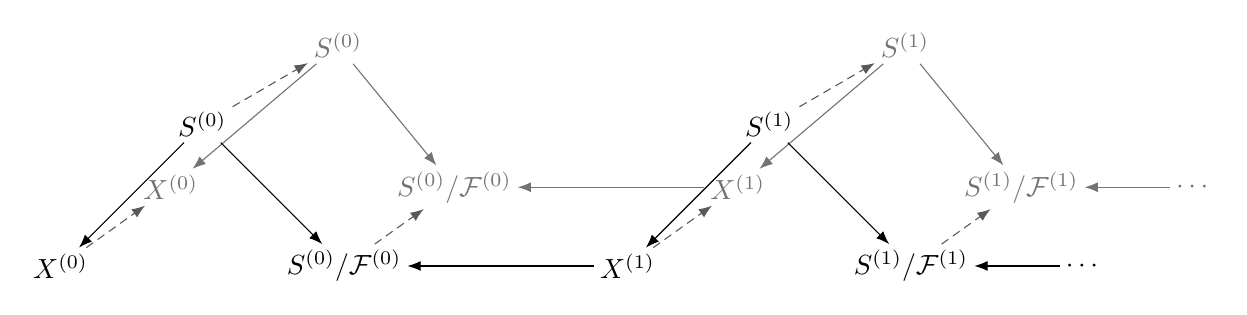
\begin{tikzpicture}[>=Latex, every node/.style={inner sep=2pt}]

  % Back copy (shifted and slightly slanted for perspective)
  \placelayer{b}{shift={(1.4,1.0)}, xslant=0.18, text=black!55}

  % Front copy
  \placelayer{f}{}

  % Internal arrows of the back copy
  \drawlayer{b}{black!55}

  % Maps from the front copy to the back copy
  \foreach \v in {X0,Q0,X1,Q1,S0,S1}
    \draw[->, densely dashed, black!65] (f\v) -- (b\v);

  % Internal arrows of the front copy
  \drawlayer{f}{black}

\end{tikzpicture}
\end{document}